\documentclass[11pt]{article}

\usepackage[margin=1in]{geometry}
\usepackage{amsmath,amssymb,amsthm,mathtools}
\usepackage{booktabs}
\usepackage{enumitem}
\usepackage{float}
\usepackage{hyperref}
\usepackage{tikz}
\usepackage{xcolor}
\usetikzlibrary{arrows.meta,positioning}

\hypersetup{colorlinks=true,linkcolor=blue!55!black,citecolor=blue!55!black,urlcolor=blue!55!black}
\setlength{\emergencystretch}{2em}

\newtheorem{theorem}{Theorem}[section]
\newtheorem{proposition}[theorem]{Proposition}
\newtheorem{corollary}[theorem]{Corollary}
\newtheorem{lemma}[theorem]{Lemma}
\theoremstyle{definition}
\newtheorem{definition}[theorem]{Definition}
\newtheorem{remark}[theorem]{Remark}

\newcommand{\F}{\mathbb F}
\newcommand{\cH}{\mathcal H}
\newcommand{\cP}{\mathcal P}
\newcommand{\cB}{\mathcal B}
\newcommand{\supp}{\operatorname{supp}}
\newcommand{\wt}{\operatorname{wt}}
\newcommand{\rank}{\operatorname{rank}}
\newcommand{\Tr}{\operatorname{Tr}}

\title{Complete Bounded Repair Ports:\\
\large Transfer, Reliability, and Geometric Structure}
\author{Tavis Rudd}
\date{July 2026}

\begin{document}
\maketitle

\begin{abstract}
For a linear code and a distinguished coordinate, the complete bounded repair
port records every dual-support recovery using at most a prescribed number of
helpers.  We keep three layers of this object visible: its support clutter, its
scalar recovery coefficients, and its reliability under helper failures.

We prove an exact weighted-functional transfer theorem for concatenation and
identify the persistent pointed obstruction to replicating a prescribed port.
Every fixed represented port satisfying this obstruction bound occurs with positive
density in an asymptotically good fixed-alphabet family.  The same object has
an exact deletion--contraction reliability calculus and a radius-truncated BEC
EXIT hierarchy whose successive differences give the cheapest available
repair radius.  At full radius, repair reliability is a specialization of the
Las Vergnas polynomial of the elementary perspective
$M\backslash x\to M/x$; the bounded-radius filtration is extra information.

Two characteristic-three families illustrate the distinction.  A
twisted-cubic--axis code has exact coordinatewise matching and transversal
rows and transfers strictly beyond the ordinary support-distance gate.  A
quartic normal rational curve with its nucleus has harmonic-quadruple circuits,
a Steiner $S(3,4,q+1)$ nucleus port, and parallel repairs at the nucleus,
whereas every curve-target repair has the nucleus as a compulsory helper.
These parallel and series geometries separate bounded-radius from full-port
information.
\end{abstract}

\section{Introduction}

Locality asks how many surviving symbols suffice to recover one unavailable
coordinate.  Availability asks for many disjoint choices of helpers.  Both
are standard in locally repairable codes
\cite{GopalanEtAl2012,PamiesEtAl2013,LavrauwVanDeVoorde2019}, but neither
describes the whole local failure event: two codes can have the same locality
and matching number while their permitted repair sets overlap very
differently.

The natural pointed object is the family of \emph{all} bounded dual-support
repairs.  We call it a complete bounded repair port.  Its matching number is
disjoint availability, its transversal number minus one is worst-case helper
failure tolerance, and its monotone Boolean function gives exact stochastic
reliability.  The coefficient layer matters as well: a repair support comes
from a scalar equation, and concatenation is controlled by the minimum cost
of realizing the corresponding block functional rather than by support alone.

For a target $x$, let $\cP_x^{(\leq r)}(C)$ be the dual words normalized by
$w_x=1$ and supported on $x$ and at most $r$ helpers.  This coefficient port
records the scalar recovery equations, not only their supports.

\begin{theorem}[MDS coefficient-port reconstruction]
\label{thm:mds-reconstruction}
Let $C\leq\F_q^E$ be an $[n,k]_q$ MDS code with $1\leq k<n$, and let
$x\in E$.  Then
\[
 \operatorname{span}\cP_x^{(\leq k)}(C)=C^\perp,
 \qquad \rho_x(C)=k,
\]
where $\rho_x(C)$ is the least reconstruction radius.  The support projection
of the minimum coefficient port is the complete $k$-uniform clutter on
$E\setminus\{x\}$.
\end{theorem}

The support clutter in this theorem is generic: it is the same for every MDS
code with these parameters.  The normalized coefficients nevertheless span
the represented dual code.  The proof chooses minimum dual words with a common
core of $k-1$ helpers and distinct private coordinates, producing a basis of
$C^\perp$.  Thus the coefficient layer retains represented information that
support-only locality discards.

Figure~\ref{fig:transfer-spine} gives the proof spine in one view.  The exact
transfer theorem concerns the first two port layers; reliability is then
determined by the transported support layer.

\begin{figure}[H]
\centering
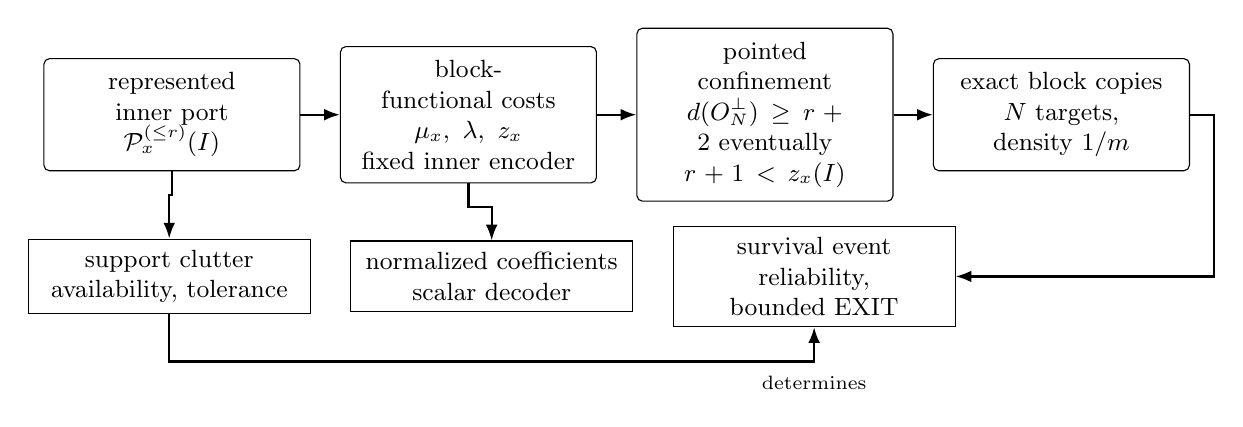
\begin{tikzpicture}[
  font=\small,
  node distance=7mm and 5mm,
  box/.style={draw, rounded corners=2pt, align=center, inner sep=5pt,
    minimum height=10mm, text width=29mm},
  view/.style={draw, align=center, inner sep=4pt, minimum height=9mm,
    text width=33mm},
  arrow/.style={-{Latex[length=2mm]}, thick}
]
\node[box] (port) {represented inner port\\$\cP_x^{(\le r)}(I)$};
\node[box, right=of port] (cost) {block-functional costs\\$\mu_x,\ \lambda,\ z_x$\\fixed inner encoder};
\node[box, right=of cost] (gate) {pointed\\confinement\\$d(O_N^\perp)\ge r+2$ eventually\\$r+1<z_x(I)$};
\node[box, right=of gate] (copies) {exact block copies\\$N$ targets, density $1/m$};

\draw[arrow] (port) -- (cost);
\draw[arrow] (cost) -- (gate);
\draw[arrow] (gate) -- (copies);

\node[view, below=of cost, xshift=-38mm] (support) {support clutter\\availability, tolerance};
\node[view, right=of support] (coeff) {normalized coefficients\\scalar decoder};
\node[view, right=of coeff] (prob) {survival event\\reliability, bounded EXIT};
\draw[arrow] (port.south) -- ++(0,-3mm) -| (support.north);
\draw[arrow] (cost.south) -- ++(0,-3mm) -| (coeff.north);
\draw[arrow] (copies.east) -- ++(3mm,0) |- (prob.east);
\draw[arrow] (support.south) -- ++(0,-6mm) -|
  node[pos=.55, below=1mm, font=\scriptsize] {determines} (prob.south);
\end{tikzpicture}
\caption{The transfer spine.  In the fixed-inner, $L$-linear concatenation
regime, weighted block-functional costs give an exact confinement gate.
When $d(O_N^\perp)\to\infty$ and $r+1<z_x(I)$, support and normalized
coefficient ports are copied into every block.  Reliability is derived from
the copied support clutter; the diagram makes no necessity claim for arbitrary
asymptotically good families.}
\label{fig:transfer-spine}
\end{figure}


The paper has six parts.  Section~\ref{sec:ports} fixes the complete pointed
object and separates support, coefficient, and probability layers.
Section~\ref{sec:transfer} gives exact and usable concatenation gates.
Section~\ref{sec:realization} turns the pointed gate into a prescribed
positive-density realization theorem.  Section~\ref{sec:reliability}
develops reliability and bounded EXIT.  Section~\ref{sec:tutte} identifies the
full-port polynomial as standard pointed-Tutte structure and isolates what the
radius filtration adds.  Section~\ref{sec:flagships} compares cubic--axis and
quartic--nucleus flagships.

The asymptotic coding ingredients, reliability identities, and pointed-Tutte
polynomial are classical.  We develop their
exact organization around the complete bounded pointed object,
together with the transfer boundary, prescribed-port consequence, and the
two exact geometric port inventories.  We make no minimum-bandwidth claim,
no full-MAP claim for a radius cutoff, and no threshold claim for harmonic
closure.
In the literature reviewed, we did not locate the exact complete-port
confinement criterion or the two coordinatewise port inventories
\cite{PamiesEtAl2013,LiuEtAl2022,GruicaEtAl2026,DavydovEtAl2021}; this is a
bounded comparison, not a priority claim.

\section{Recovery sets and normalized equations}
\label{sec:recovery-equations}

Let $C\leq\F_q^E$ be a linear code.  We first separate four layers that are
often harmlessly conflated when only locality is at issue.

Fix a target $x\in E$ and a helper bound $r$.  A dual word $w\in C^\perp$
with $w_x\ne0$ gives
\[
 c_x=\sum_{y\ne x}-\frac{w_y}{w_x}c_y
 \qquad(c\in C).
\]
Its exact helper support is $\supp(w)\setminus\{x\}$.  Define
\[
 \cH_x^{(\le r)}(C)=
 \{\supp(w)\setminus\{x\}:w\in C^\perp, w_x\ne0,
       \wt(w)\le r+1\}.
\]
The usual bounded recovery-set family is the upward closure of
$\cH_x^{(\le r)}(C)$ inside the subsets of $E\setminus\{x\}$ of size at most
$r$.  Its inclusion-minimal members form the minimal recovery-set clutter.
Thus exact supports, recovery sets, and minimal recovery sets are distinct
but determine the same monotone success event.

The coefficient layer is
\[
 \cP_x^{(\le r)}(C)=
 \{w\in C^\perp:w_x=1, \wt(w)\le r+1\}.
\]
These normalized recovery equations determine their exact supports, while
the converse generally fails.  The operational model is scalar exact repair:
each participating helper supplies one symbol of $\F_q$.  Array-code access,
subpacketization, and repair bandwidth are different optimization problems
\cite{ShahEtAl2010,YeBarg2016,KurzYaakobi2021}.

If $A\subseteq E\setminus\{x\}$ is the surviving helper set, put
\[
 f_{x,r}(A)=1
 \quad\Longleftrightarrow\quad
 \text{$A$ contains a member of $\cH_x^{(\le r)}(C)$}.
\]
Under independent helper survival with probabilities $(s_y)$, the bounded
repair reliability is
\[
 R_{x,r}((s_y))=\mathbb E[f_{x,r}].
\]
It depends only on the minimal recovery sets, but it is not determined by
their minimum cardinality.  Section~\ref{sec:separations} shows that even the
complete relative-weight hierarchy does not determine the corresponding
bounded reliability law.

For several target coordinates, a recovery equation is a dual subspace rather
than one dual word.  Let $P\subseteq E$, $J=E\setminus P$, and let
$G=(G_P\mid G_J)$ be a full-row-rank generator matrix.  If
$T\leq\operatorname{im}G_P$ is a subspace of target linear combinations, a
normalized recovery system for $T$ consists of linear maps
\[
 \alpha:T\longrightarrow\F_q^P,
 \qquad
 \beta:T\longrightarrow\F_q^J
\]
such that
\[
 G_P\alpha=\operatorname{id}_T,
 \qquad
 G_J\beta=-\operatorname{id}_T.
\]
For each $t\in T$, the vector $(\alpha(t),\beta(t))$ is then a dual word.
The map $\alpha$ records the chosen target normalization and $\beta$ records
the helper coefficients.

The helper union of the system is the support of $\beta(T)$:
\[
 \supp(\beta(T))=
 \{j\in J:\text{some }t\in T\text{ has }\beta(t)_j\ne0\}.
\]
Its helper cost is $|\supp(\beta(T))|$.  We call a target subspace internally
recoverable when it lies in
\[
 W_P=\operatorname{im}G_P\cap\operatorname{im}G_J.
\]
Only this recovered subspace dimension is counted below.  Relations supported
entirely on $P$ have recovered dimension zero and do not consume helpers.

For later comparison, the normalized equations at one coordinate reconstruct
the represented code at radius $r$ when their span is $C^\perp$.  The least
such $r$ is the reconstruction radius.

\begin{theorem}[MDS reconstruction from minimum-weight recovery equations]
\label{thm:mds-reconstruction}
\coverage{absent}%
Let $C\leq\F_q^E$ be an $[n,k]_q$ MDS code with $1\leq k<n$, and let
$x\in E$.  Then
\[
 \operatorname{span}\cP_x^{(\leq k)}(C)=C^\perp,
\]
the reconstruction radius is $k$, and the supports of the minimum-weight
recovery equations form the complete $k$-uniform clutter on
$E\setminus\{x\}$.
\end{theorem}

\begin{proof}
The dual has dimension $n-k$ and minimum distance $k+1$.  For every
$(k+1)$-set $T\subseteq E$, restriction of $C^\perp$ to $E\setminus T$ has
domain dimension $n-k$ and codomain dimension $n-k-1$.  Its kernel contains a
nonzero word supported on $T$, and the distance bound forces its support to be
all of $T$.  Hence the exact helper supports through $x$ are precisely the
$k$-subsets of $E\setminus\{x\}$.

Choose a fixed $(k-1)$-set $Q\subseteq E\setminus\{x\}$.  For every
$t\in E\setminus(\{x\}\cup Q)$, choose the normalized minimum dual word
supported on $\{x,t\}\cup Q$.  Evaluation at the private coordinates $t$
shows that these $n-k$ words are independent.  They are therefore a basis of
$C^\perp$.  No smaller radius contains a nonzero normalized equation, again
by the dual-distance bound.
\proves{thm:mds-reconstruction}%
\end{proof}

The support clutter in this theorem depends only on the MDS parameters.  The
normalized equations retain the represented dual code.  This is the first
instance of the support--coefficient distinction used in the transfer and
separation results below.

\section{Puncturing, shortening, and relative recovery costs}
\label{sec:relative-weights}

The local problem forgets the outer code and asks how many helpers realize
a prescribed target combination.  In the running example, the helper
coefficient vectors $(1,0,0,0)$, $(0,1,0,0)$, and $(0,0,1,1)$ all realize
$u$.  Their differences lie in the kernel of the helper generator map.
Passing to its quotient identifies the requested combination while leaving
the cost of its different physical realizations to be minimized.

Continue with $G=(G_P\mid G_J)$, viewed as
$G_P:\F_q^P\to\F_q^k$ and $G_J:\F_q^J\to\F_q^k$, and set
\[
 U_P=\operatorname{im}G_P,
 \qquad
 W_P=U_P\cap\operatorname{im}G_J,
\]
\[
 K_P=\ker G_J,
 \qquad
 D_P=G_J^{-1}(U_P).
\]
\begin{proposition}[Associated nested code pair]
\label{prop:associated-pair}
\coverage{complete}%
\lean{helper_ker_le_helperCodeForTargetSpace,%
map_helperCodeForTargetSpace_eq_recoverableTargetMessageSpace,%
recoverableTargetMap_surjective,%
mem_ker_recoverableTargetMap_iff}%
Restriction of $G_J$ gives an exact sequence
\begin{equation}
 0\longrightarrow K_P\longrightarrow D_P
 \xrightarrow{G_J}W_P\longrightarrow0.
 \label{eq:associated-exact-sequence}
\end{equation}
\end{proposition}

\begin{proof}
By definition, $K_P=\ker G_J$ is contained in
$D_P=G_J^{-1}(U_P)$.  The kernel of the restricted map is therefore $K_P$.
Its image is
\[
 G_J(D_P)=\operatorname{im}G_J\cap U_P=W_P,
\]
so the restricted map is onto $W_P$.
\proves{prop:associated-pair}%
\end{proof}

The first isomorphism theorem applied to the restricted map gives
$D_P/K_P\cong W_P$.

\begin{proposition}[Canonical puncturing--shortening description]
\label{prop:puncture-shorten-pair}
\coverage{absent}%
With puncturing and shortening taken onto the helper set $J$,
\begin{equation}
 D_P=\operatorname{punct}_J(I^\perp),
 \qquad
 K_P=\operatorname{short}_J(I^\perp).
 \label{eq:puncture-shorten-pair}
\end{equation}
Thus $\operatorname{punct}_J$ restricts to $J$, while
$\operatorname{short}_J$ first requires the coordinates on $P$ to vanish and
then restricts to $J$.  These operations are dual to one another.  Taking
duals inside $\F_q^J$ gives
\begin{equation}
 D_P^\perp=\operatorname{short}_J(I),
 \qquad
 K_P^\perp=\operatorname{punct}_J(I).
 \label{eq:dual-puncture-shorten-pair}
\end{equation}
Consequently the nested pair depends only on the code $I$ and the split
$E=P\sqcup J$; changing the row basis of a generator matrix leaves it
unchanged.
\end{proposition}

\begin{proof}
A vector $a\in\F_q^J$ lies in $\operatorname{punct}_J(I^\perp)$ exactly when
some $p\in\F_q^P$ satisfies $G_Pp+G_Ja=0$, equivalently
$G_Ja\in\operatorname{im}G_P$, which is $a\in D_P$.  It lies in
$\operatorname{short}_J(I^\perp)$ exactly when $(0,a)\in I^\perp$,
equivalently $G_Ja=0$, which is $a\in K_P$.
The dual identities follow from the standard puncturing--shortening duality.
\proves{prop:puncture-shorten-pair}%
\end{proof}

Thus a monomial relabeling of helpers gives the corresponding monomially
equivalent pair, while a row-basis change does nothing to the pair itself.

For a subspace $A\leq\F_q^J$, write $\supp A$ for the union of the supports
of its vectors.  For nested linear codes $K\subseteq D\leq\F_q^J$, the $t$th relative
generalized Hamming weight is
\[
 M_t(D,K)=
 \min\{ |\supp L|:L\leq D,
     \dim L-\dim(L\cap K)=t\}.
\]
Equivalently, one may minimize over subspaces disjoint from $K$ and of
dimension $t$.  Strict growth and the relative Singleton bound are
Proposition~2 and Theorem~4 of Luo et al.~\cite{LuoEtAl2005}; standard
treatments also cover ordinary Wei duality and computational forms
\cite{GeilEtAl2014,SanJose2025}.
For nested code pairs in linear secret sharing, RDLPs and RGHWs already give
exact information and reconstruction thresholds
\cite{KuriharaUyematsuMatsumoto2012}.

The following result is the standard nested-code support invariant applied to
the canonical puncturing--shortening pair, with the normalization and helper
support correspondence stated in recovery language.

\begin{theorem}[Relative weights are exact recovery costs]
\label{thm:relative-weight-recovery}
\coverage{absent}%
Let $\ell=\dim W_P$ and $1\leq t\leq\ell$.  The minimum helper-union size
among recovery systems for all helper-recoverable $t$-dimensional
subspaces of target linear combinations, denoted $\mu_t(P)$, is
\[
 \mu_t(P)=M_t(D_P,K_P).
\]
More precisely, after forgetting the target normalization, normalized recovery
systems of recovered dimension $t$ are in support-preserving correspondence
with subspaces
\[
 L\leq D_P,\qquad \dim L=t,\qquad L\cap K_P=0,
\]
while normalization on the chosen recovered subspace $T\leq W_P$ is a linear
section of $G_P$ over $T$.
\end{theorem}

\begin{proof}
Let a normalized system recover a $t$-dimensional subspace $T\leq W_P$.
In the notation of Section~\ref{sec:recovery-equations}, put $L=\beta(T)$.
Since $G_J\beta=-\operatorname{id}_T$, the map $\beta$ is injective,
$L\leq D_P$, and $L\cap K_P=0$.  Moreover $G_JL=T$, and the union of
helpers in the system is exactly $\supp L$.

Conversely, let $L\leq D_P$ have dimension $t$ and meet $K_P$ trivially.
Then $G_J|_L$ is an isomorphism from $L$ onto the $t$-dimensional subspace
$T=G_JL\leq W_P$.  Choose a linear section
$\alpha:T\to\F_q^P$ with $G_P\alpha=\operatorname{id}_T$.  Put
$\beta=-(G_J|_L)^{-1}$.  Then
$G_P\alpha+G_J\beta=0$, so $(\alpha,\beta)$ is a normalized recovery system
with helper union $\supp L$.

It remains to compare this minimum with the standard relative-weight
definition.  If $L'\leq D_P$ satisfies
\[
 \dim L'-\dim(L'\cap K_P)=t,
\]
choose a vector-space complement $L$ to $L'\cap K_P$ inside $L'$.  Then
$\dim L=t$, $L\cap K_P=0$, and $\supp L\subseteq\supp L'$.  The reverse
inclusion of feasible classes is immediate.  The two minima are equal.
\uses{prop:associated-pair}%
\proves{thm:relative-weight-recovery}%
\end{proof}

The corresponding relative dimension/length profile is
\[
 K_s(D_P,K_P)=
 \max_{\substack{H\subseteq J\\|H|=s}}
 \bigl(\dim(D_P\cap\F_q^H)-\dim(K_P\cap\F_q^H)\bigr),
\]
where $\F_q^H$ denotes vectors supported on $H$.

\begin{proposition}[Recovery interpretation of the relative profile]
\label{prop:relative-profile}
\coverage{absent}%
For $0\leq s\leq|J|$,
\[
 K_s(D_P,K_P)=
 \max_{\substack{H\subseteq J\\|H|=s}}
 \dim\bigl(W_P\cap\operatorname{span}(G_H)\bigr).
\]
Consequently,
\[
 M_t(D_P,K_P)=\min\{s:K_s(D_P,K_P)\geq t\}.
\]
Thus $K_s$ is the maximum number of independent target linear combinations
recoverable from a fixed budget of $s$ helpers.
\end{proposition}

\begin{proof}
Fix $H$.  Restrict the exact map~\eqref{eq:associated-exact-sequence} to
$D_P\cap\F_q^H$.  Its kernel is $K_P\cap\F_q^H$, and its image is
$W_P\cap\operatorname{span}(G_H)$.  Rank--nullity gives the first equality
after maximizing over $H$.  The second is the standard inverse relation
between the relative dimension/length profile and relative generalized
weights; it also follows directly from Theorem~\ref{thm:relative-weight-recovery}.
\uses{prop:associated-pair, thm:relative-weight-recovery}%
\proves{prop:relative-profile}%
\end{proof}

Standard shortening--puncturing duality gives the complementary failure
interpretation: the relative weights of
$D_P^\perp\subseteq K_P^\perp$ are the minimum numbers of helper failures
that leave prescribed dimensions of $W_P$ ambiguous
\cite{LuoEtAl2005,GeilEtAl2014}.

The strict inequalities
\[
 1\leq M_1(D_P,K_P)<\cdots<M_\ell(D_P,K_P)
\]
therefore say that each additional independent target combination requires a
strictly larger helper union.  These minima solve the single-block problem but
do not yet provide recursive state: the next section restores the functional
labels needed for exact concatenation.  Only when an outer-distance condition
removes every nonzero label does the answer collapse to
$M_t(D_P,K_P)+d(I^\perp)$.

\subsection{Prescribed quotient operations}

The pair construction admits a useful general form.  For finite linear codes
$K\subseteq D\leq\F_q^E$, let $\pi:D\to D/K$ be the quotient map.
Given a finite $\F_q$-space $T$ and a linear map $B:T\to D/K$, put
\[
 \kappa_T^{D/K}(B)=
 \min_{\substack{Y:T\to D\ \mathrm{linear}\\\pi Y=B}}
 |\supp Y(T)|.
\]
Thus a quotient label specifies an operation and a lift specifies its
physical coordinates.  Under $D_P/K_P\cong W_P$, the inclusion of a
target subspace $T$ has cost $\rho_T(I)$, the least helper-union size
for recovering $T$ in $I$: its helper lift has image under
$G_J$ equal to the requested target, and negating the helper coefficients
gives the normalized dual equations.  More generally, minimizing
$\kappa_T^{D/K}(B)$ over injective $B$ with $\dim T=t$ gives $M_t(D,K)$.
Indeed an injective quotient image forces the lift image to be disjoint
from $K$, and every $t$-dimensional subspace disjoint from $K$ supplies
such a map after choosing a basis.

\begin{theorem}[Composition of quotient-labelled lifts]
\label{thm:quotient-lifting-composition}
\coverage{absent}%
Let $E_i$ be disjoint, let $K_i\subseteq D_i\leq\F_q^{E_i}$, and write
$\pi_i:D_i\to L_i=D_i/K_i$.  For a nested pair
$R_0\subseteq R_1\leq\bigoplus_iL_i$, take inverse images inside
$\bigoplus_iD_i$:
\[
 \pi=\bigoplus_i\pi_i,\qquad D=\pi^{-1}(R_1),\qquad K=\pi^{-1}(R_0).
\]
Then $D/K\cong R_1/R_0$.  Writing $\bar\pi:R_1\to R_1/R_0$, every
linear $B:T\to R_1/R_0$ satisfies
\begin{equation}
 \kappa_T^{D/K}(B)=
 \min_{\substack{Z:T\to R_1\ \mathrm{linear}\\\bar\pi Z=B}}
 \sum_i\kappa_T^{D_i/K_i}(\operatorname{pr}_iZ).
 \label{eq:quotient-lifting-composition}
\end{equation}
Minimizing lifts compose to a witness.  Repeated substitution is associative.
\end{theorem}

\begin{proof}
The surjection $D\to R_1/R_0$ induced by $\pi$ has kernel $K$, giving
the asserted isomorphism.  A lift $Y:T\to D$ determines $Z=\pi Y$ with
$\bar\pi Z=B$.  For fixed $Z$, its block maps $Y_i$ are precisely the
independent lifts of $\operatorname{pr}_iZ$.  Their supports are disjoint,
so their minimum costs add.  All quotient maps admit linear sections;
hence these minima are attained and their block witnesses assemble to a
lift of $B$.  This proves both inequalities in the formula.  At further
levels, either order of substitution minimizes over the same compatible
intermediate maps and the same sum of leaf costs.
\proves{thm:quotient-lifting-composition}%
\end{proof}

No common extension field is needed here.  For heterogeneous injective
encoders $e_i:V_i\hookrightarrow\F_q^{E_i}$ and a base-field-linear
outer relation $O\leq\bigoplus_iV_i$, the interface is
$e_i^*:\F_q^{E_i}\to V_i^*$ and compatibility is membership in
$\operatorname{ann}(O)$.  Orthogonality to all encoded outer words proves
this directly.  Target-normalized fibres retain their target constraints
and exclude target coordinates from the cost.  To identify a prescribed
target with the full alphabet $V_j$, the projection $O\to V_j$ must be
surjective; a nonzero projection alone is insufficient.  With nonzero $T$
and at least two blocks, the zero-functional nonconfinement contribution is
$\rho_{j,T}+\min_{i\ne j}d(I_i^\perp)$, by adjoining a minimum dual word
in the cheapest external block.  Extension-field scalar and projective
actions used below are additional structure of that specialization.

\paragraph{Available quotient directions.}
For a coordinate set $A\subseteq E$, the quotient directions realizable
entirely on $A$ form
\[
 L(A)=\pi(D\cap\F_q^A),\qquad
 \dim L(A)=\dim(D\cap\F_q^A)-\dim(K\cap\F_q^A).
\]
Here $\F_q^A$ is embedded by zero-extension.  The formula is rank--nullity
for the restricted quotient map.  A prescribed $B$ has a lift on $A$
exactly when $B(T)\subseteq L(A)$, since the restricted surjection admits
a linear section.  This retains the directions exposed on $A$, as well as
their maximum possible rank; minimizing ordinary words of $D$ would lose
the requirement that the quotient label be nonzero.

\section{Exact confinement under concatenation}
\label{sec:confinement}

Two confinement results govern the section.  Classifying recovery systems by
their outer functional labels gives the exact equation escape cost
(Theorem~\ref{thm:ungated-ranked-confinement}).  Deleting dispensable external
coefficients instead gives minimal-support transfer under a target-touching
distance hypothesis (Theorem~\ref{thm:minimal-support-confinement}).  The latter
transfers availability and support-based allocations even when equations can
escape.  Finally, the full label-indexed costs pass to the next concatenation
level by an associative min--sum law.

\paragraph{Represented inner code.}
Let $L/\F_q$ be a finite extension and let
$\iota:L\xrightarrow{\sim} I\leq\F_q^E$ be an $\F_q$-linear isomorphism,
used as the inner encoder.
Assume $0<\dim I<|E|$.
Whenever the outer alphabet $L$ occurs below, $I$ denotes the represented
inner code $(I,\iota)$, not only its image subspace.  In particular,
$O\circ I$, $\Phi_I$, $\lambda_{I,T}$, $\mu_{I,P,T}$, and
$\Gamma_{j,T}(O,I)$ depend on $\iota$.  The earlier pair
$K_P\subseteq D_P$ depends only on the image code and target/helper split.
Proposition~\ref{prop:functional-label-separation} shows that this distinction
cannot be suppressed under concatenation.

For an $L$-linear outer code $O\leq L^N$, write
\[
 O\circ I=\{(\iota(a_1),\ldots,\iota(a_N)):(a_1,\ldots,a_N)\in O\}.
\]
Each block has a label map
\[
 \underbrace{\F_q^E}_{\text{inner coefficients}}
 \xrightarrow{\ \Phi_I\ }
 \underbrace{L^*}_{\text{functional label}},
\qquad
\Phi_I(y)(a)=\langle y,\iota(a)\rangle.
\]
Here $L^*=\operatorname{Hom}_{\F_q}(L,\F_q)$.  The chosen message coordinates
identify each earlier generator column with the functional
$a\mapsto\iota(a)_e$; equivalently, it is the unique trace coefficient $b_e$
with $\iota(a)_e=\operatorname{Tr}_{L/\F_q}(b_ea)$.  We transport $T$ and
$G_P\alpha=\operatorname{id}_T$ through this same identification.
Two coefficient vectors receive the same label precisely when they differ by
an inner dual word, because $\ker\Phi_I=I^\perp$.  The prescribed-coset costs
below record the cheapest coefficient support in each fibre of this map.

\paragraph{Outer compatibility.}
A block vector
$y=(y_1,\ldots,y_N)$ belongs to $(O\circ I)^\perp$ precisely when
\begin{equation}
 (\Phi_I(y_1),\ldots,\Phi_I(y_N))\in
 \operatorname{FD}(O),
 \label{eq:block-functional-dual}
\end{equation}
where
\[
 \operatorname{FD}(O)=
 \{(\beta_j)\in(L^*)^N:\textstyle\sum_j\beta_j(a_j)=0
       \text{ for every }(a_j)\in O\}.
\]
Indeed, both conditions say that $y$ is orthogonal to every encoded outer
word.  Write $\beta_j(a)=\operatorname{Tr}_{L/\F_q}(b_ja)$.  The functional-dual
condition becomes
\[
 \operatorname{Tr}_{L/\F_q}\!\left(\sum_j b_ja_j\right)=0
 \qquad\text{for every }(a_j)\in O.
\]
Because $O$ is $L$-linear, the same holds after multiplying $(a_j)$ by every
$\lambda\in L$.  Nondegeneracy of the trace pairing then forces
$\sum_jb_ja_j=0$.  Hence $(b_j)\in O^\perp$, and the converse is immediate.
This identification preserves block support, so the support distance of
$\operatorname{FD}(O)$ is $d(O^\perp)$.

\paragraph{Confinement and target normalization.}
Fix a target block and a nonzero target-message subspace $T\leq U_P$.  A
system is \emph{confined} if every one of its equations is supported in that
target block.  Let
$\rho_T(I)$ be the minimum helper-union size of a normalized recovery system
for $T$ in the inner code, with value $\infty$ when no such system exists.
Thus $\rho_T(I)<\infty$ exactly when $T\leq W_P$.  In a concatenation, a
normalized system for $T$ means a linear family of dual equations whose
target-block coefficient map $\alpha:T\to\F_q^P$ satisfies
$G_P\alpha=\operatorname{id}_T$ under the fixed inner-message
identification.  This fixes a normalization condition, not a particular
section $\alpha$: the admissible sections vary in the minimization.
This agrees with the intrinsic target image of the
concatenated generator whenever the outer projection onto the chosen block is
surjective.  In particular, $d(O^\perp)>1$ guarantees surjectivity: an
$L$-linear coordinate image is either $0$ or $L$, and a zero image would put a
weight-one word in $O^\perp$.

For an $\F_q$-linear map $B:T\to L^*$, define
\begin{equation}
 \lambda_{I,T}(B)=
 \min_{\substack{Y:T\to\F_q^E\ \mathrm{linear}\\
                  \Phi_IY=B}}
 |\supp Y(T)|.
 \label{eq:ordinary-joint-coset-cost}
\end{equation}
For the target block, define
\begin{equation}
 \mu_{I,P,T}(B)=
 \min_{\substack{\alpha:T\to\F_q^P,\ \beta:T\to\F_q^J\ \mathrm{linear}\\
                  G_P\alpha=\operatorname{id}_T\\
                  \Phi_I(\alpha,\beta)=B}}
 |\supp\beta(T)|.
 \label{eq:target-joint-coset-cost}
\end{equation}
An empty minimum is $\infty$.  After choosing a basis of $T$,
\eqref{eq:ordinary-joint-coset-cost} is the minimum union support of
representatives of prescribed cosets of $I^\perp$.  This is the fixed-instance
quantity underlying generalized coset weights and generalized covering radii
\cite{ZhangEtAl2019,ElimelechFirerSchwartz2021}.  The target version retains
the normalization required by the recovery problem.  In particular,
\begin{equation}
 \mu_{I,P,T}(0)=\rho_T(I).
 \label{eq:zero-target-joint-coset-cost}
\end{equation}
For each equation parameter $t\in T$, the value $B(t)$ is exactly the outer
functional label induced by that equation in the block.

Let
\[
 \mathcal B_T(O)=
 \operatorname{Hom}_{\F_q}\bigl(T,\operatorname{FD}(O)\bigr).
\]
For $B\in\mathcal B_T(O)$, write $B=(B_h)_{h=1}^N$ with
$B_h:T\to L^*$.  Assume $N\geq2$, fix a target block $j$ whose coordinate projection
$O\to L$ is nonzero, hence surjective, and put
\begin{equation}
 \begin{split}
 \Gamma_{j,T}(O,I)=\min\Biggl\{&
 \mu_{I,P,T}(0)+d(I^\perp),\\
 &\min_{0\ne B\in\mathcal B_T(O)}
 \left(
 \mu_{I,P,T}(B_j)+
 \sum_{h\ne j}\lambda_{I,T}(B_h)
 \right)
 \Biggr\}.
 \end{split}
 \label{eq:weighted-subspace-cost}
\end{equation}

\begin{theorem}[Exact nonconfinement cost from labelled coset supports]
\label{thm:ungated-ranked-confinement}
\coverage{absent}%
\imports{Zhang:tuple-coset-support}%
Under the hypotheses above, $\Gamma_{j,T}(O,I)$ is the least helper-union
size of a nonconfined normalized recovery system for $T$ in $O\circ I$, with
value $\infty$ if no such system exists.
Thus every cost-$\leq r$ system for $T$ is confined if and only if
\begin{equation}
 r<\Gamma_{j,T}(O,I).
 \label{eq:weighted-subspace-gate}
\end{equation}
For $1\leq t\leq\ell=\dim W_P$, set
\begin{equation}
 \Gamma_{j,t}(O,I)=
 \min_{\substack{T\leq W_P\\\dim T=t}}\Gamma_{j,T}(O,I).
 \label{eq:ranked-weighted-cost}
\end{equation}
Then every cost-$\leq r$ system for every helper-recoverable
$t$-dimensional target subspace is confined if and only if
$r<\Gamma_{j,t}(O,I)$.  Below either threshold, restriction and zero-extension
are inverse bijections on normalized systems and preserve exact helper
supports.
\end{theorem}

\begin{proof}
Write a recovery system as an $\F_q$-linear map
$Y:T\to(O\circ I)^\perp$ and let $Y_h$ be its block maps.  By
\eqref{eq:block-functional-dual},
\[
 B_h=\Phi_IY_h
\]
defines a linear map $B:T\to\operatorname{FD}(O)$.  Conversely, compatible
linear lifts of the block maps of any such $B$ give a map into the
concatenated dual.  At the target block, compatibility with the chosen target
space is exactly the constraint in~\eqref{eq:target-joint-coset-cost}.

Suppose first that $B\ne0$.  No nonzero element of
$\operatorname{FD}(O)$ is supported only at $j$: testing such an element
against outer words whose $j$th coordinate ranges over $L$ would force its
$j$th functional to vanish.  Hence some block map $B_h$ with $h\ne j$ is
nonzero, and every lift is nonconfined.  Distinct inner blocks have disjoint
helper coordinates, so the minimum helper union for this fixed $B$ is
\[
 \mu_{I,P,T}(B_j)+
 \sum_{h\ne j}\lambda_{I,T}(B_h).
\]
The block lifts can be chosen independently, so this lower bound is attained.

If $B=0$, every block map takes values in $I^\perp=\ker\Phi_I$.  The target
block costs $\rho_T(I)=\mu_{I,P,T}(0)$.  Nonconfinement requires a nonzero map
$T\to I^\perp$ in another block.  Its image has union support at least
$d(I^\perp)$, and equality is attained by $u\mapsto f(u)v$, where
$0\ne f\in T^*$ and $v$ is a minimum-weight word of $I^\perp$.

The zero and nonzero functional sectors are exhaustive, proving
\eqref{eq:weighted-subspace-cost} and~\eqref{eq:weighted-subspace-gate}.
Minimizing over $t$-dimensional $T$ proves the ranked statement.  Below the
first nonconfined cost, every global system has zero coefficient maps in all
blocks outside $j$.  Restriction therefore preserves its target normalization
and helper support.  Conversely, zero-extending an inner dual system remains
orthogonal to every concatenated word, so the two operations are inverse with
coefficients and supports unchanged.
\proves{thm:ungated-ranked-confinement}%
\end{proof}

\paragraph{The running example: equations versus useful repairs.}
For the code in the introduction,
$G=(e_1\mid e_1,e_1,e_2,e_1+e_2)$.
Its inner-dual distance is two: two repeated columns give a weight-two
relation, and no column is zero.  The local recovery cost for $u$ is one.
Identify its message space with $L=\F_4$ and take $O=L^N$, $N\geq2$.
There are no nonzero outer-dual labels, so the exact formula gives
$\Gamma_{j,1}=1+2=3$.  A cost-three nonconfined equation adds the relation
$u+u=0$ in another block to the local recovery of $u$.
Deleting those two external coefficients leaves the original repair.

Nevertheless every minimal repair remains in its own block at every radius:
the outer messages are independent, so external coefficients cannot supply
any part of the target functional.  The three local choices remain
$\{1\}$, $\{2\}$, and $\{3,4\}$.  This example exhibits the zero sector
of the exact formula and the difference between its coefficient threshold
and the operational theorem below.  The nonzero-sector alignment obstruction
is exhibited separately in Proposition~\ref{prop:functional-label-separation}.

\subsection{Minimal supports and operational transfer}

An external equation can violate coefficient confinement without supplying a
new recovery option.  To separate these questions, let
$\mathcal M_{j,T}^{(\leq r)}(O\circ I)$ be the inclusion-minimal helper
supports recovering $T$ with at most $r$ helpers.  A set recovers $T$ when
some normalized system uses only that set.  Define the target-touching distance
\[
 \delta_j(O^\perp)=\min\{\wt(u):u\in O^\perp,\ u_j\ne0\},
\]
with empty minimum $\infty$.

\begin{theorem}[Minimal-support confinement]
\label{thm:minimal-support-confinement}
\coverage{absent}%
Let $O\leq L^N$ be $L$-linear, let its projection onto block $j$ be
surjective, and let $0\ne T\leq U_P$.  If $\delta_j(O^\perp)>r+1$, then
\[
 \mathcal M_{j,T}^{(\leq r)}(O\circ I)
 =\{\{j\}\times H:H\in\mathcal M_T^{(\leq r)}(I)\}.
\]
No inequality involving $\rho_T(I)+d(I^\perp)$ is required.
Consequently bounded recovery success has the same probability for every
global helper-availability law with the prescribed target-block marginal.
\end{theorem}

\begin{proof}
Let $Y$ be a normalized system with helper support $H$, $|H|\leq r$, and
put $B_h=\Phi_IY_h$.  If $B_j\ne0$, choose $v\in T$ with $B_j(v)\ne0$.
The trace identification sends $B(v)$ to an outer dual word touching $j$.
Its other nonzero blocks each contain a helper in $H$, so its weight is at
most $r+1$, a contradiction.  Thus $B_j=0$, and the target-block portion
of $Y$ is an inner-dual system with the same target normalization.  Deleting
all external coefficients preserves recovery and only decreases support.
Every global minimal support is therefore local.  Conversely, a proper
globally recovering subset of a local minimal support would, by this same
restriction argument, contradict local minimality.  Zero-extension supplies
the other inclusion.  For each available set, success means containing one
of these minimal supports; the two success indicators therefore agree
pointwise after restriction to the target block.  Taking expectations proves
the probability assertion without an independence assumption.
\proves{thm:minimal-support-confinement}%
\end{proof}

The first new external repair has its own threshold.  Let
$\varepsilon_{j,T}$ be the least size of a globally recovering helper set
$H$ whose portion in block $j$ does not recover $T$ locally.  Equivalently,
it is the least size of a global minimal support using an external helper:
minimize inside $H$ for one direction; a local recovery inside a minimal
support contradicts minimality for the other.  The theorem gives
$\varepsilon_{j,T}\geq\delta_j(O^\perp)-1$ when the latter is finite,
and $\varepsilon_{j,T}=\infty$ when $\delta_j(O^\perp)=\infty$.
Its value cannot be obtained simply by deleting the zero sector from
$\Gamma_{j,T}$: a nonzero-labelled lift can also contain a local recovery.
For $O=L^N$, every minimal recovery support is local at every radius,
although adjoining an external inner-dual word gives the finite equation
threshold $\rho_T(I)+d(I^\perp)$ whenever $T$ is locally recoverable.

\subsection{Repeated concatenation}

The ordinary prescribed-coset costs retain the intermediate labels needed at
the next concatenation level.  Target-normalized composition also retains the
part of each intermediate label already supplied by target coordinates.  In
schematic form,
\[
 \text{cost of output label}
 =\min_{\text{compatible intermediate labels}}
   \sum_{\text{inner blocks}}\text{inner realization cost}.
\]
The eliminated variables are the intermediate labels shared by adjacent
levels.  The resulting formulas are instances of variable elimination over
the min-sum semiring \cite{AjiMcEliece2000}.  This is also the algebraic
form of passing symbol-indexed inner costs to an outer decoder, as in soft and
generalized-concatenated decoding \cite{GuruswamiSudan2002,BlomqvistEtAl2020}.

The zero-functional nonconfinement cost alone is not compositional.  The next
separation holds the underlying binary code and all its unlabelled recovery
data fixed.

\begin{proposition}[Unlabelled data do not determine finite composition]
\label{prop:functional-label-separation}
\coverage{absent}%
Over $\F_2\subseteq\F_4$, there are two represented inner encoders with the
same image code, dual code, target/helper nested pair, complete relative-weight
hierarchy, dual distance, unlabelled normalized helper-support family, and
zero-functional nonconfinement costs for every recoverable target subspace, but one
fixed outer represented code gives different exact nonconfinement costs.
\end{proposition}

\begin{proof}
Write the nonzero elements of $\F_4$ as
$1,\omega,\omega^2=1+\omega$ and take generator columns
\[
 I_1:(1,1,\omega),
 \qquad
 I_2:(1,1,\omega^2),
\]
with the first coordinate targeted.  Relative to the binary basis
$(1,\omega)$ of $\F_4$, each displayed field element is a two-dimensional
binary generator column.  Both generator matrices have binary row
space
\[
 \{(x,x,y):x,y\in\F_2\}
\]
and dual $\langle(1,1,0)\rangle$.  Thus both have dual distance $2$,
$K_P=0\subseteq D_P=\langle(1,0)\rangle$, $M_1=1$, and the same unique
minimal helper support.  Their recoverable target space is one-dimensional,
so their complete zero-functional profile is the common value $1+2=3$.

For this table identify a column $c$ with the functional
$a\mapsto\Tr(\omega^2ca)$.  This is the coordinate-dot-product pairing
in the basis $(1,\omega)$; the corresponding trace coefficient is
$\omega^2c$.  The common rescaling preserves every outer $L$-linear dual
subspace.  In this column-label order $(1,\omega,\omega^2)$, the ordinary coset costs are
$(1,1,2)$ for $I_1$ and $(1,2,1)$ for $I_2$; the normalized target costs are
respectively $(0,2,1)$ and $(0,1,2)$.  Take the fixed outer code whose
functional dual is the line spanned by $(1,\omega)$.  Its nonzero multiples
have target label $s$ and external label $s\omega$.  The complete calculation
is
\[
\begin{array}{c|cc|ccc|ccc}
 s & s & s\omega
   & \mu_1(s) & \lambda_1(s\omega) & \text{total}
   & \mu_2(s) & \lambda_2(s\omega) & \text{total}\\ \hline
 1        & 1        & \omega   & 0&1&1 & 0&2&2\\
 \omega   & \omega   & \omega^2 & 2&2&4 & 1&1&2\\
 \omega^2 & \omega^2 & 1        & 1&1&2 & 2&1&3
\end{array}
\]
Equation~\eqref{eq:weighted-subspace-cost} therefore gives exact costs $1$
and $2$.  Only the alignment of costs with the intermediate functional labels
has changed.
\uses{thm:ungated-ranked-confinement}%
\proves{prop:functional-label-separation}%
\end{proof}

Let $\F_q\subseteq L\subseteq M$ be a tower of finite fields.  Let $B$ be an
$\F_q$-linear represented code with message space $L$, and let $A$ be an
$L$-linear represented code with message space $M$.  The composite $A\circ B$
replaces each coordinate of an $A$-word by its represented $B$-block.
After identifying a functional with its unique trace coefficient, write their
dual restriction maps as
\[
 \phi_B:\F_q^{E_B}\longrightarrow L,
 \qquad
 \phi_A:L^{E_A}\longrightarrow M.
\]
For an $\F_q$-space $T$ and $b:T\to L$, put
\[
 \Lambda_{B,T}(b)=
 \min_{\phi_BY=b}|\supp Y(T)|.
\]
Define $\Lambda_{A,T}$ and $\Lambda_{A\circ B,T}$ similarly.  If
$J\subseteq E_B$, let $\Lambda_{B,J,T}$ denote the same minimum with $Y$
supported on $J$ and $\phi_B$ restricted to those coordinates.
Thus $\phi$ is the trace-coordinate form of $\Phi$, and $\Lambda$ is the
corresponding ordinary prescribed-coset cost $\lambda$.  The change of letters
only distinguishes the two levels in the following substitution.

For the recovery-specific form, suppose that a target set in $A\circ B$ meets
block $e$ in $P_e\subseteq E_B$.  Put $J_e=E_B\setminus P_e$ and
$U_{P_e}=\operatorname{im}\phi_{B,P_e}$.  If $T\leq M$, let
$\iota_T:T\hookrightarrow M$ be the inclusion.  The variables below have the
following roles:
\[
\begin{array}{c|l}
 U_e & \text{intermediate contribution supplied by target coordinates in block }e\\
 X_e & \text{total intermediate functional label required in block }e\\
 X_e-U_e & \text{label that the helper coordinates in block }e\text{ must realize.}
\end{array}
\]

\begin{theorem}[Min--sum closure of prescribed-coset support costs]
\label{prop:prescribed-coset-composition}
\coverage{absent}%
\imports{Zhang:tuple-coset-support,Aji:distributive-law}%
\uses{thm:ungated-ranked-confinement}%
For every $\F_q$-linear map $c:T\to M$, the ordinary prescribed-coset cost is
\begin{equation}
 \Lambda_{A\circ B,T}(c)=
 \min_{\substack{X:T\to L^{E_A}\ \phi_AX=c}}
 \sum_{e\in E_A}\Lambda_{B,T}(X_e).
 \label{eq:coset-cost-composition}
\end{equation}
For $T\leq M$ and the target split above, the target-normalized recovery cost
is
\begin{equation}
 \mu_{A\circ B,P,T}(c)=
 \min_{\substack{U,X:T\to L^{E_A}\\
                  U_e(T)\subseteq U_{P_e}\ (e\in E_A)\\
                  \phi_AU=\iota_T,\ \phi_AX=c}}
 \sum_{e\in E_A}\Lambda_{B,J_e,T}(X_e-U_e).
 \label{eq:target-cost-composition}
\end{equation}
Both formulas iterate associatively through a finite tower: either
parenthesization minimizes over the same intermediate labels and target
contributions and sums the same leaf costs.  Storing minimizing target and
helper lifts propagates one coefficient-level witness; retaining every witness
requires the full lift sets rather than only the numerical minima.
\end{theorem}

\begin{proof}
A leaf-level lift $Y:T\to\F_q^{E_A\times E_B}$ determines intermediate maps
$X_e=\phi_BY_e$.  Its support is the disjoint union of its supports in the
inner blocks.  At fixed $X$, the block lifts are independent and attain their
minima separately, which proves \eqref{eq:coset-cost-composition}.

For the target-normalized formula, lift $U_e$ to an actual target map
$a_e:T\to\F_q^{P_e}$.  The condition $\phi_AU=\iota_T$ is exactly target
normalization.  Once $X_e$ is fixed, the helper contribution must lift
$X_e-U_e$ through $\phi_{B,J_e}$, independently in each block.  This proves
\eqref{eq:target-cost-composition}; storing the displayed lifts gives the
stated witness semantics.  At three or more levels, either parenthesization
eliminates the same intermediate arrays and target contributions, proving
associativity.
\uses{thm:ungated-ranked-confinement}%
\proves{prop:prescribed-coset-composition}%
\end{proof}

\paragraph{Sharp scalar envelopes.}
The full labelled function gives simple bounds when only its smallest and
largest nonzero values are retained.  When $T\ne0$, set
\[
 \delta_{B,T}=\min_{0\ne b:T\to L}\Lambda_{B,T}(b),
 \qquad
 R_{B,T}=\max_{0\ne b:T\to L}\Lambda_{B,T}(b).
\]
For $c\ne0$, the exact formula has the sharp coarsening
\begin{equation}
 \delta_{B,T}\Lambda_{A,T}(c)
 \leq \Lambda_{A\circ B,T}(c)
 \leq R_{B,T}\Lambda_{A,T}(c).
 \label{eq:coset-cost-envelope}
\end{equation}
Neither constant can be improved without further hypotheses.
Indeed, every nonzero intermediate coordinate map costs between
$\delta_{B,T}$ and $R_{B,T}$.  Minimizing the number of nonzero intermediate
coordinates proves the bounds; a one-coordinate outer realization attaining
either extremum proves sharpness.

\paragraph{Dual-distance recursion.}
The same zero/nonzero-label split gives
\begin{equation}
 d((A\circ B)^\perp)=
 \min\left\{
 d(B^\perp),
 \min_{0\ne z\in A^\perp}
 \sum_{e\in E_A}\Lambda_{B,\F_q}(u\mapsto uz_e)
 \right\}.
 \label{eq:dual-distance-composition}
\end{equation}
A word in $(A\circ B)^\perp$ either has zero intermediate label, when a
minimum word of $B^\perp$ in one block is optimal, or has a nonzero label
$z\in A^\perp$, when the block representatives minimize independently.  This
proves \eqref{eq:dual-distance-composition}.

\paragraph{Tower consequence.}
Substituting these recursively computed costs into
\eqref{eq:weighted-subspace-cost} gives the exact nonconfinement cost through
any finite tower, with the zero and nonzero functional sectors kept separate
at every level.

The trace identifications in these formulas are compatible with the tower.
Write $\iota_A:M\to A\leq L^{E_A}$ for the represented encoder of $A$.
For $v\in T$ and $m\in M$, trace transitivity gives
\[
 \sum_e\Tr_{L/\F_q}\bigl(X_e(v)\,\iota_A(m)_e\bigr)
 =\Tr_{M/\F_q}\bigl(\phi_A(X(v))m\bigr),
\]
and nondegeneracy of the trace pairing identifies the composite restriction
map with $\phi_A\circ\phi_B^{E_A}$, where $\phi_B^{E_A}$ applies $\phi_B$
blockwise.

\paragraph{Simultaneous confinement in every dimension.}
\begin{corollary}[Rank-one criterion for complete bounded transfer]
\label{cor:all-rank-bottleneck}
\coverage{absent}%
For every target block $j$ with nonzero outer projection,
\begin{equation}
 \min_{0\ne T\leq W_P}\Gamma_{j,T}(O,I)=\Gamma_{j,1}(O,I).
 \label{eq:all-rank-bottleneck}
\end{equation}
For every integer $r\geq0$, the following are equivalent:
\begin{enumerate}
 \item every cost-$\leq r$ system on every helper-recoverable target line
 is confined;
 \item every cost-$\leq r$ system on every nonzero helper-recoverable
 target subspace is confined; and
 \item $r<\Gamma_{j,1}(O,I)$.
\end{enumerate}
Under these conditions, restriction and zero-extension are inverse bijections
simultaneously for every nonzero $T\leq W_P$, preserving every coefficient and
exact helper support through radius $r$.

Consequently, any statistic defined solely from these bounded systems and
invariant under this bijection is preserved.  In particular, the bounded
reliability laws and the capacity and scheduling regions defined later from
their coefficients or supports agree.  Targetwise and rankwise minimum costs
also agree after truncation $c\mapsto\min\{c,r+1\}$ (with
$\min\{\infty,r+1\}=r+1$).  If every relevant inner minimum is at most $r$,
then the untruncated minima agree as well.
\end{corollary}

\begin{proof}
If a system on $0\ne T\leq W_P$ is nonconfined, some external block map is
nonzero on a vector $u\in T$.  Restriction to $\langle u\rangle$ remains
nonconfined and cannot enlarge its helper union.  This proves the displayed
equality, and Theorem~\ref{thm:ungated-ranked-confinement} gives the three
equivalent conditions.  When they hold, every bounded system is confined, so
restriction deletes only zero external blocks and zero-extension is its
inverse.  The coefficient, support, reliability, capacity, and scheduling
assertions follow from this bijection.  For a minimum helper-union cost, either
the inner minimum is at most $r$ and the bijection gives equality, or both
inner and concatenated minima exceed $r$; this is precisely equality after
truncation at $r+1$.
\uses{thm:ungated-ranked-confinement}%
\proves{cor:all-rank-bottleneck}%
\end{proof}

\section{Reliability and bounded EXIT}
\label{sec:reliability}

Let $\cH$ be a repair clutter on helper set $V$.  For $v\in V$, define
\[
 \cH-v=\min\{E\in\cH:v\notin E\},
 \qquad
 \cH/v=\min\{E\setminus\{v\}:E\in\cH\}.
\]

\begin{theorem}[Reliability calculus]
\label{thm:reliability}
For independent helper survival probabilities $(s_v)$,
\[
 R_\cH(s)=(1-s_v)R_{\cH-v}(s)+s_vR_{\cH/v}(s),
\]
and
\[
 \frac{\partial R_\cH}{\partial s_v}
 =R_{\cH/v}-R_{\cH-v}
 =\Pr(v\text{ is pivotal}).
\]
Under homogeneous survival $s$,
$R_\cH'(s)=\sum_v\Pr_s(v\text{ is pivotal})$.
If the minimum blocker size is $\tau$ and there are $b_\tau$ minimum
blockers, then for helper failure probability $p$,
\[
 1-R_\cH(1-p)=b_\tau p^\tau+O(p^{\tau+1}).
\]
\end{theorem}

\begin{proof}
Write \(f_\cH(A)=1\) when \(A\) contains an edge of \(\cH\), and write it as
zero otherwise.  The reliability is the finite multilinear sum
\[
 R_\cH(s)=\sum_{A\subseteq V}f_\cH(A)
 \prod_{y\in A}s_y\prod_{y\notin A}(1-s_y).
\]
Partition the subsets according to whether they contain \(v\).  Erasing \(v\)
from those that do contain it identifies the two parts with the Boolean
systems \(\cH-v\) and \(\cH/v\), respectively.  This gives
\[
 R_\cH=(1-s_v)R_{\cH-v}+s_vR_{\cH/v}.
\]
The two conditional reliabilities do not involve \(s_v\), so differentiation
gives \(R_{\cH/v}-R_{\cH-v}\).  Monotonicity makes this difference the
conditional probability that adjoining \(v\) changes failure into success,
which is precisely pivotality.  On the diagonal \(s_v=s\), the chain rule
sums these coordinate derivatives and gives the Russo--Margulis identity.

Now expose the failed set \(F\).  Repair fails exactly when \(F\) is a
transversal of \(\cH\), equivalently when it contains a minimal blocker.
Thus
\[
 1-R_\cH(1-p)=
 \sum_{\substack{F\subseteq V\\F\ {\rm is\ a\ transversal}}}
 p^{|F|}(1-p)^{|V|-|F|}.
\]
There are no summands below degree \(\tau\), and the transversals of size
\(\tau\) are exactly the \(b_\tau\) minimum blockers.  Their contribution is
\(b_\tau p^\tau(1-p)^{|V|-\tau}
=b_\tau p^\tau+O(p^{\tau+1})\).  Every remaining term contains at least
\(p^{\tau+1}\); the sum is finite, proving the expansion.
\end{proof}

These are the standard deletion--contraction and pivotality identities for a
monotone reliability system \cite{Colbourn1987}.

For EXIT conventions, condition the target $x$ unavailable and erase helper
$v$ with probability $p_v$.  Put
\[
 h_x^{(\leq r)}(p)=\Pr(f_x^{(\leq r)}(A)=0),
 \qquad R_x^{(\leq r)}=1-h_x^{(\leq r)}.
\]
This is an \emph{extrinsic} failure probability.  If the target is itself
erased with probability $p_x$, its residual erasure probability is
$p_xh_x^{(\leq r)}$.  At full radius it is symbol-MAP EXIT; at finite radius
it is a bounded-query decoder and carries no capacity claim
\cite{AshikhminKramerTenBrink2004,Mazumdar2023}.

\begin{proposition}[Bounded-EXIT hierarchy]
\label{prop:bounded-exit}
The failure form of deletion--contraction is
\[
 h_\cH(p)=p_vh_{\cH-v}(p)+(1-p_v)h_{\cH/v}(p),
 \qquad
 \frac{\partial h_\cH}{\partial p_v}
 =\Pr(v\text{ is pivotal}).
\]
If $L_x(A)$ is the size of the cheapest repair contained in the realized
survivor set, with $L_x=\infty$ when none exists, then
\[
 \Pr(L_x=r)=h_x^{(\leq r-1)}-h_x^{(\leq r)},
 \qquad
 \Pr(L_x=\infty)=h_x^{\rm MAP}.
\]
The first identity is for \(r\geq1\).
\end{proposition}

\begin{proof}
Conditioning on whether \(v\) is erased gives the displayed recurrence:
when it is erased, only repairs avoiding \(v\) remain; when it survives, it
may be contracted from every repair.  Equivalently, substitute
\(s_y=1-p_y\) in the reliability recurrence and take complements.
Differentiation reverses both signs, so the derivative is again the pivotal
probability.

Let \(\cH_x^{(\leq r)}\) be the full port filtered by edge size at most \(r\).
The event \(L_x\leq r\) is exactly success for this truncated port.  Hence
\[
 \{L_x=r\}=\{L_x>r-1\}\setminus\{L_x>r\},
\]
and taking probabilities gives the difference of failure curves.  At full
radius, the complementary event is that no repair exists, which is
\(L_x=\infty\).
\end{proof}

Minimal transversals of $\cH_x^{(\leq r)}$ are exact target-specific,
one-shot bounded-repair failure certificates.  They are not automatically
the representation-dependent stopping sets of a global iterative Tanner
decoder.

For a length-$N$ code define the radius-$r$ locality deficit
\[
 L_r(x)=\int_0^1\bigl(h_x^{(\leq r)}(p)-h_x^{\rm MAP}(p)\bigr)\,dp.
\]
If $\Delta a_k$ counts size-$k$ survivor sets repaired by full MAP but not at
radius $r$, beta integration gives
\[
 L_r(x)=\sum_{k=0}^{N-1}
 \frac{\Delta a_k}{N\binom{N-1}{k}}.
\]
With entropy normalized in $\log_q$ units, the unrecoverable-symbol indicator
is the normalized conditional entropy on the $q$-ary erasure channel.  Under
this convention the symbol-MAP areas sum to the code dimension $K$
\cite{AshikhminKramerTenBrink2004}, so
\[
 \sum_x\int_0^1h_x^{(\leq r)}(p)\,dp
 =K+\sum_xL_r(x).
\]

\section{Pointed Tutte structure}
\label{sec:tutte}

Let $M$ be the column matroid of a projective-system code on
$E=V\sqcup\{x\}$, with $x$ neither a loop nor a coloop.  Put
\[
 \epsilon_x(A)=r_M(A\cup\{x\})-r_M(A)\in\{0,1\}.
\]
The set $A$ repairs $x$ exactly when $\epsilon_x(A)=0$.

\begin{theorem}[Pointed perspective polynomial]
\label{thm:tutte}
Let $D=M\backslash x$ and $Q=M/x$.  The Las Vergnas polynomial of the
elementary perspective $D\to Q$ is
\[
 T_{D\to Q}(X,Y,Z)=
 \sum_{A\subseteq V}
 (X-1)^{r(M)-r_M(A\cup\{x\})}
 (Y-1)^{|A|-r_M(A)}Z^{\epsilon_x(A)}.
\]
If
\[
 S_x(u)=\sum_{\epsilon_x(A)=0}u^{|A|},
\]
then, for $n=|V|$,
\[
 R_{(M,x)}(s)=
 \sum_{\epsilon_x(A)=0}s^{|A|}(1-s)^{n-|A|}.
\]
Consequently, when $s\ne1$,
\[
 R_{(M,x)}(s)=(1-s)^nS_x\!\left(\frac{s}{1-s}\right).
\]
Writing $U_K(u,y)=\sum_Au^{|A|}y^{r_K(A)}$, one also has
\[
 S_x(u)=\left.\frac{\partial}{\partial y}
 \bigl(U_D(u,y)-U_Q(u,y)\bigr)\right|_{y=1}.
\]
\end{theorem}

\begin{proof}
Contraction gives
$r_D(A)=r_M(A)$ and $r_Q(A)=r_M(A\cup\{x\})-1$, so
$r_D(A)-r_Q(A)=1-\epsilon_x(A)$.  Substitution in the rank-one
perspective expansion gives the displayed polynomial term by term.  The
$Z^0$ terms are exactly the successful sets; more explicitly, for $u\ne0$,
\[
 S_x(u)=u^{r(M)}[Z^0]T_{D\to Q}(1+u^{-1},1+u,Z),
\]
because a term with exponents $a,b,0$ has
$|A|=r(M)-a+b$.  Multiplying the coefficient of $u^{|A|}$ by
$s^{|A|}(1-s)^{n-|A|}$ and summing gives the reliability formula.
Finally,
\[
 \left.\partial_y(y^{r_D(A)}-y^{r_Q(A)})\right|_{y=1}
 =r_D(A)-r_Q(A),
\]
which is one when $\epsilon_x(A)=0$ and zero when
$\epsilon_x(A)=1$.  Summing the differentiated terms proves the last
identity.
\end{proof}

This identification is the singleton specialization of standard set-pointed
Tutte theory \cite[equation~(3.1)]{LasVergnas1999}; it is not a new polynomial.
\begin{corollary}[Pointed repair--failure duality]
\label{cor:pointed-duality}
Pointed duality gives
\[
 R_{(M,x)}(s)+R_{(M^*,x)}(1-s)=1,
\]
and the minimal failure blockers of $(M,x)$ are exactly the minimal repair
sets of $(M^*,x)$.  For a represented matroid they are the sets
$Q'\setminus\{x\}$, where $Q'$ ranges over cocircuits containing $x$;
equivalently, $Q'$ is an inclusion-minimal row-code support through $x$.
In particular,
\[
 \tau_{\rm full}(x)=d_x(C)-1,
 \qquad
 d_x(C)=\min\{\wt(c):c\in C,\ c_x\neq0\}.
\]
\end{corollary}

\begin{proof}
For $F\subseteq V$, put $A=V\setminus F$.  The dual rank formula, applied
once to $F$ and once to $F\cup\{x\}$, gives
\[
 r_{M^*}(F\cup\{x\})-r_{M^*}(F)=1-\epsilon_x(A).
\]
Thus $F$ repairs $x$ in $M^*$ exactly when its complement fails to repair
$x$ in $M$.  Complementation preserves the product measure after replacing
$s$ by $1-s$, which proves the reliability identity.  It also exchanges
minimal dual repairs with minimal primal failure blockers.  Circuits of
$M^*$ are cocircuits of $M$, so the blockers are $Q'\setminus\{x\}$ for
cocircuits $Q'$ through $x$.  In a represented matroid, cocircuits are the
inclusion-minimal nonzero row-code supports.  Taking the smallest support
through $x$ proves the distance formula.
\end{proof}

\begin{lemma}[Sparse-paving pointed enumerator]
\label{lem:sparse-paving-profile}
For a rank-$r$ sparse paving matroid on $n$ elements with distinguished
element $x$, the multiplicity enumerator of the rank triples
\(
 (r_M(A),r_M(A\cup\{x\}),|A|)
\), over all \(A\subseteq E\setminus\{x\}\), is determined by $n,r$, the
number of circuit-hyperplanes containing $x$, and the number avoiding $x$.
Equivalently, these data determine the full pointed-perspective polynomial.
They do not determine the labeled subset-rank function \(A\mapsto r_M(A)\).
\end{lemma}

\begin{proof}
Every set of size below $r$ is independent, every set of size above $r$ has
full rank, and an $r$-set has rank $r-1$ exactly when it is a
circuit-hyperplane.  Hence the rank triple
\[
 \bigl(r_M(A),r_M(A\cup\{x\}),|A|\bigr),\qquad
 A\subseteq E\setminus\{x\},
\]
has its uniform-matroid value except when $A$ or $A\cup\{x\}$ is one of the
two indicated types of circuit-hyperplane.  Their two counts therefore
determine the multiplicity of every rank triple.
\end{proof}

\begin{proposition}[The radius filtration is not a pointed-Tutte specialization]
\label{prop:filtration-boundary}
The complete pointed polynomial does not determine the bounded-radius
reliability filtration, even among rank-four systems represented over
$\F_7$.
\end{proposition}

\begin{proof}
The mechanism is sparse paving.  Lemma~\ref{lem:sparse-paving-profile} does
not record how the circuit-hyperplanes through $x$ meet after $x$ is removed.
The radius-$(r-1)$ reliability does record those intersections, because it is
the probability of the union of their containment events.

Distinguish column $0$ in each of the following matrices; columns $1,\ldots,6$
are the helpers:
\[
 G_{\rm dis}=
 \begin{pmatrix}
 1&1&1&1&0&1&1\\
 0&3&1&4&0&6&1\\
 0&2&3&2&1&5&0\\
 0&1&4&1&2&4&3
 \end{pmatrix},
 \qquad
 G_{\rm ov}=
 \begin{pmatrix}
 1&1&1&1&1&1&1\\
 0&1&2&5&4&0&6\\
 0&4&2&0&2&1&2\\
 0&4&1&6&4&5&4
 \end{pmatrix}.
\]
All entries and determinants below are in $\F_7$.  Every three-column set
is independent.  The dependent four-column sets are, respectively,
\[
 \{0145,0236,2345\},
 \qquad
 \{0123,0256,3456\}.
\]
Here, for example, $0145$ denotes $\{0,1,4,5\}$.  Direct elimination gives
the two lists: all other four-column minors are nonzero, and every triple
extends to one of them.  The complete determinant ledger and exact replay
are recorded in Appendix~\ref{sec:seed-evidence}.  Thus each displayed
representation has rank four, has no circuit of size at most three, and has
exactly the three listed circuit-hyperplanes.

Both matroids are rank-four sparse paving matroids with three
circuit-hyperplanes, two through the distinguished column and one avoiding
it.  The preceding sparse-paving count therefore gives, for both systems,
\[
\begin{split}
T(X,Y,Z)={}&(X-1)^3Z+6(X-1)^2Z+15(X-1)Z+2(X-1)\\
&+18Z+(Y-1)Z+14+6(Y-1)+(Y-1)^2.
\end{split}
\]
Equivalently, their complete successful-set enumerators are both
\[
 2u^3+14u^4+6u^5+u^6.
\]

At radius three, however, the minimal repairs are
\[
 \{145,236\}\quad\hbox{for }G_{\rm dis},
 \qquad
 \{123,256\}\quad\hbox{for }G_{\rm ov}.
\]
The first pair is disjoint and the second pair meets in helper $2$.
Inclusion--exclusion under homogeneous survival consequently gives
\[
 R_{\rm dis}^{(\leq3)}(s)=2s^3-s^6,
 \qquad
 R_{\rm ov}^{(\leq3)}(s)=2s^3-s^5.
\]
The pointed polynomials agree while the filtered curves do not.
\end{proof}

\begin{theorem}[Matched asymptotic bounded-port separation]
\label{thm:asymptotic-separation}
There are two asymptotically good fixed-alphabet linear-code families
$C_N^{\rm dis},C_N^{\rm ov}$ over $\F_7$ with the following properties.
For every $N$ the families have the same length and dimension, and they have
the same proved lower bound on minimum distance.  Each family has a
designated coordinate class of density exactly $1/7$.  At every target in
that class, for all sufficiently large $N$, the radius-three repair port is
a copy of the corresponding port in
Proposition~\ref{prop:filtration-boundary}.  In particular,
\[
 R_{\rm dis}^{(\leq3)}(s)=2s^3-s^6,\qquad
 R_{\rm ov}^{(\leq3)}(s)=2s^3-s^5.
\]
The two seed ports have the same pointed rank-triple multiplicity enumerator,
locality three, and two minimum repairs.  Their availability is not matched:
it is two for the disjoint seed and one for the overlapping seed.
\end{theorem}

\begin{proof}
Let $I_{\rm dis}$ and $I_{\rm ov}$ be the row-span codes of the two displayed
matrices.  Both have parameters $[7,4,3]_7$.  Indeed, their rank is four.
A listed circuit-hyperplane supplies a hyperplane containing four columns,
so the primal distance is at most three; no five columns have rank at most
three, so it is exactly three.  Every triple is independent and a dependent
four-set exists, hence
\[
 d(I_{\rm dis}^{\perp})=d(I_{\rm ov}^{\perp})=4.
\]
In each seed a listed circuit-hyperplane through $0$ supplies a weight-four
dual word through the target.  Therefore the zero-functional pointed fiber
cost is both at least and at most four, and
\[
 z_0(I_{\rm dis})=z_0(I_{\rm ov})=4+4=8.
\]
The radius-three transfer gate is consequently $3+1<8$ for both seeds.

Put $L=\F_{7^4}$ and choose one asymptotically good $L$-linear outer family
$O_N\leq L^N$ whose dual distance tends to infinity; the standard random
linear-code argument quoted after Corollary~\ref{cor:mds-fingerprints}
supplies such a family with both primal and dual relative distances positive.
Use the two inner encoders with this same $O_N$.  If $O_N$ has dimension
$K_N$ and distance $D_N$, Proposition~\ref{prop:concat-parameters} gives,
for both concatenations,
\[
 n_N=7N,\qquad k_N=4K_N,\qquad d_N\geq3D_N.
\]
Thus their global formulas and asymptotic bounds agree.

Since $d(O_N^\perp)\to\infty$, Theorem~\ref{thm:prescribed} applies
simultaneously to the two fixed inner codes.  For every sufficiently large
$N$ and every block $j$, it identifies the complete radius-three support and
coefficient ports at $(j,0)$ with the corresponding seed ports.  These $N$
targets among $7N$ coordinates have density exactly $1/7$.  Literal port
equality preserves the two reliability polynomials computed in
Proposition~\ref{prop:filtration-boundary}.  The same proposition and
Lemma~\ref{lem:sparse-paving-profile} give the assertions about the seed
profiles, locality, repair count, and the unmatched matching numbers.
\end{proof}

\begin{corollary}[Synthesis under exact port transfer]
\label{cor:transfer-synthesis}
Whenever Theorem~\ref{thm:prescribed} transfers a radius-$r$ support and
coefficient port exactly, it simultaneously transfers every smaller support
filtration and every normalized decoder in that range.  Consequently it
preserves matching and transversal numbers, minimal blockers and their
leading failure terms, multivariate reliability, and every bounded-EXIT
curve through radius $r$.  Any difference between two inner ports in one of
these quantities therefore persists on their designated positive-density
target classes.
\end{corollary}

\begin{proof}
For each $t\leq r$, the radius-$t$ port is obtained from the radius-$r$ port
by retaining precisely the witnesses with at most $t$ helpers.  The
zero-extension bijection in Theorem~\ref{thm:prescribed} preserves supports,
coefficients, and cardinality, so it commutes with every such truncation.
Matching numbers, transversal numbers, and minimal blockers depend only on
the resulting clutter.  Reliability is the finite product-measure sum over
its upward closure, the leading failure term is determined by its minimum
blockers, and bounded EXIT is the complementary reliability under
$s_v=1-p_v$.  Each claimed consequence therefore follows from literal
equality after relabeling.
\end{proof}

The retained field-nine harmonic computation gives a geometric instance of
the same boundary: six-element circuits in a rank-five code add five-helper
repairs beyond the classified radius-four port.  It illustrates the effect
but is not evidence for Proposition~\ref{prop:filtration-boundary}.

\section{Geometric flagships}
\label{sec:flagships}

\subsection{The twisted-cubic--axis family}

Let $q=3^h$ and work in $\mathrm{PG}(3,q)$.  Put
\[
 T_q=\{C(t)=(1:t:t^2:t^3):t\in\F_q\},
\]
\[
 L_q=\{A(u)=(0:1:u:0):u\in\F_q\}
 \cup\{A_\infty=(0:0:1:0)\}.
\]
The line $L_q$ is the characteristic-three axis of the osculating-plane
pencil \cite{DavydovEtAl2021}; all statements below follow directly from
the displayed coordinates.

\begin{theorem}[Cubic--axis port]
\label{thm:cubic}
The row code on $T_q\sqcup L_q$ is $[2q+1,4,q-1]_q$.  Its minimal circuits
of size at most four are the triples on $L_q$ and the sets
\[
 \{C(s),C(t),C(u),(0:e_1:e_2:0)\}
\]
for distinct $s,t,u$, where $e_1=s+t+u$ and
$e_2=st+su+tu$.  Every cubic coordinate has
\[
 (\nu,\tau)=\left(\frac{q-1}{2},q-2\right).
\]
If $Z_3(q)$ is the maximum size of a three-term-zero-sum-free subset of
$(\F_q,+)$, then
\[
 (\nu,\tau)_{A_\infty}
 =\left(\frac{5q-3}{6},2q-1-Z_3(q)\right),
\]
\[
 (\nu,\tau)_{A(a)}
 =\left(\frac{5q-9}{6},2q-2-Z_3(q)\right).
\]
In particular every coordinate satisfies $\tau>\nu$ for $q\geq9$.
\end{theorem}

\begin{proof}
A plane containing $L_q$ contains at most one cubic point by Frobenius
injectivity; a plane not containing it meets the line once and the cubic at
most three times.  This gives the code parameters.  Vandermonde determinants
classify the displayed small circuits.  At an axis target the repair clutter
is a disjoint union of $K_q$ and a zero-sum-triple hypergraph, so matching and
transversal numbers add; complements of transversals are precisely
zero-sum-free sets.  At a cubic target, inversion relabels the other cubic
helpers by $\F_q^*$.  A multiplicative-generator pairing gives $(q-1)/2$
repairs with distinct axis completions; no larger matching is possible because
each repair uses two of the $q-1$ cubic helpers.  The shifted-inverse
complement lemma bounds a repair-free helper set by $q+2$, attained by all
axis helpers together with one cubic helper.  Taking complements gives
$\tau=q-2$.  The stated strict inequalities follow from the elementary bound
$Z_3(q)\leq q-2$ and the displayed formulas.
\end{proof}

Restoring the cubic point at infinity gives a
$[2q+2,4,q]_q$ code whose full minimal port is visible at radius four and has
uniform rows
\[
 \left(\frac{q-1}{2},q-1\right)\text{ on the cubic},
 \qquad
 \left(\frac{5q-3}{6},2q-3\right)\text{ on the axis}.
\]
This is the inner code in the strict weighted-transfer example above.
The exact $q=9$ rows are recorded in Appendix~\ref{sec:finite-evidence}.

\subsection{The quartic--nucleus harmonic family}

Let
\[
 V(t)=(1,t,t^2,t^3,t^4),\qquad V(\infty)=e_4,
 \qquad N=e_2,
\]
and let $S_q=\{V(t):t\in\mathbb P^1(\F_q)\}\cup\{N\}$.
The classical normal-rational-curve nucleus formula identifies $N$ as the
hyperplane nucleus in characteristic three \cite[Theorem~1]{GmainerHavlicek2013}.

\begin{theorem}[Quartic--nucleus port]
\label{thm:harmonic}
For $q=3^h\geq9$, the row code $Q_q$ on $S_q$ has parameters
\[
 [q+2,5,q-3]_q,\qquad d(Q_q^\perp)=5.
\]
Its minimal circuits of size at most five are exactly
\[
 \{N\}\cup B,
\]
where $B$ is a harmonic quadruple of $\mathbb P^1(\F_q)$.  These quadruples
form a Steiner system $S(3,4,q+1)$, the characteristic-three four-set orbit
in the standard $\operatorname{PGL}(2,q)$ design construction
\cite[Section~2]{Tricot2024}.  Hence the radius-four repairs are all
$B$ at the nucleus and all $\{N\}\cup(B\setminus\{x\})$ at a curve target
$x\in B$.  The nucleus has
\[
 \frac{(q+1)q(q-1)}{24}
\]
radius-four repairs, and every curve target has $q(q-1)/6$.  Every curve
target has $(\nu,\tau)=(1,1)$.
\end{theorem}

\begin{proof}
For distinct finite $a,b,c,d$, the hyperplane through their quartic columns
contains $N$ exactly when $e_2(a,b,c,d)=0$; with $\infty$ present the condition
is $a+b+c=0$.  Given three finite points, if $e_1=a+b+c\neq0$, the unique
completion is $d=-e_2/e_1$; if $e_1=0$, the unique completion is $\infty$.
In the first case, substituting $d=a$, for example, changes the harmonic
equation to $(a-b)(a-c)=0$, and similarly for $b$ and $c$; hence the
completion is distinct.  In the second case, writing $c=-a-b$ gives
$e_2(a,b,c)=-(a-b)^2\neq0$, so no finite completion exists.  A triple
$\{\infty,a,b\}$ has the unique completion $-a-b$, distinct from $a,b$
in characteristic three.  This proves the Steiner property.  Since
$\{\infty,0,1,-1\}$ is one block and $\operatorname{PGL}(2,q)$ is
3-transitive, unique completion also identifies the blocks with its
projective orbit.

Any five curve points are independent by the extended Vandermonde
determinant.  Expanding the determinant of $N,V(a),V(b),V(c),V(d)$ along
the nucleus row gives
\[
 \Delta(a,b,c,d)e_2(a,b,c,d),
\]
and with infinity present it gives $\Delta(a,b,c)e_1(a,b,c)$.  The
Vandermonde factor is nonzero for distinct parameters.  Thus
$\{N\}\cup B$ is dependent exactly for a harmonic block.  A complementary
minor shows that $N$ with any three distinct curve points is independent;
in the zero-sum finite branch its determinant reduces to
$-\Delta(a,b,c)e_2(a,b,c)$, which is nonzero by the calculation above.
Deleting any point therefore restores independence.  These are all circuits
of size at most five, so the dual distance is five.

A nonzero hyperplane restricts to a nonzero polynomial of degree at most four
on the normal rational curve, counting infinity as a root when the quartic
coefficient vanishes.  It therefore contains at most four curve points.  If
it also contains $N$, equality occurs exactly on a harmonic block, so the
largest section of $S_q$ has five points.  Hence the primal distance is
$(q+2)-5=q-3$.  Finally, the Steiner count is
$\binom{q+1}{3}/\binom43$, and the number of blocks through a fixed curve
point is $\binom q2/\binom32$.  The circuit--repair correspondence gives the
stated ports and counts.
\end{proof}

The inner-dual half of the coarse transfer gate is automatic at radius four
because $5<2d(Q_q^\perp)=10$.  Theorem~\ref{thm:prescribed} therefore places the
entire harmonic port with positive density in asymptotically good
fixed-$\F_q$ families.

\subsection{Reliability, EXIT, and the geometric contrast}

The nucleus repairs are the blocks of the Steiner system
\(S(3,4,q+1)\).  At a curve target, every radius-four repair contains the
nucleus.  Thus the nucleus port is a parallel family of four-helper repairs,
whereas the curve port has a compulsory series helper.  The reliability and
bounded-EXIT theorem applies to both ports without an exact finite profile.
Exact field-nine profiles are computational refinements recorded in
Appendix~\ref{sec:finite-evidence}; they are not used in the body theorem chain.

Finally, the harmonic small-circuit closure has a deterministic nucleus gate.
Let $D(S)$ close curve set $S$ under ``three points of a harmonic block add
the fourth.''  Then
\[
 \operatorname{cl}_4(S)=S\quad\text{if $S$ contains no block},
\qquad
 \operatorname{cl}_4(S)=\{N\}\cup D(S)\quad\text{otherwise},
\]
and $\operatorname{cl}_4(S\cup\{N\})=\{N\}\cup D(S)$.
Indeed, without $N$ no curve point can be repaired, while a complete block
$B\subseteq S$ repairs $N$.  Once $N$ is present, the curve-target repairs
are exactly $N$ together with three points of a harmonic block, so iteration
is precisely harmonic completion.  This proves all three identities.

Appendix~\ref{sec:finite-evidence} gives a field-nine block-free rank-five
spanning set and its one-round completion after adjoining $N$.  These witnesses
illustrate the nucleus gate but are not inputs to the closure identities, an
asymptotic propagation claim, or a threshold theorem.

\section{Conclusion}

Functional labels make local recovery costs composable: fixing the
intermediate operations separates the block fibres, and retaining their
lifts reconstructs the recovery coefficients.  The resulting exact equation
threshold includes external dual perturbations that create no useful repair
alternative.  Target-touching outer dual distance gives the stronger
operational conclusion: every bounded minimal recovery support remains local,
so reliability and capacity-constrained allocations transfer without the
additional inner-dual distance restriction.

The downstream question determines what the optimizer must retain.
Numerical costs suffice for their declared contexts; support alternatives
preserve reweighting, availability, and helper sharing.  Ergodis embodies
these distinctions in executable recovery choices and checked optimization
bounds.  The remaining algorithmic challenge is to construct the required
interfaces economically, including local compilation and certification,
rather than merely evaluate them after they have been built.


\appendix
\section{Verification scope}
\label{sec:verification}

Every mathematical result has a human proof independent of software execution.
The paper-owned Lean companion additionally verifies the associated-pair
exact sequence
\[
 0\longrightarrow K_P\longrightarrow D_P
 \xrightarrow{\,G_J\,}W_P\longrightarrow0.
\]
Its formal coverage stops there: the relative-weight identity, confinement
and composition theorems, operational consequences, and examples are not
established by that companion.  The claim manifest records this distinction
statement by statement.  The four checked declarations, pinned toolchain,
Mathlib revision, and axiom inventory are documented in the companion's
\texttt{lean/README.md} and \texttt{verification/README.md}.

Ergodis's independent checkers validate specified finite composition and
transition contracts.  Relating a source recovery problem to such a checked
presentation requires justification of the lowering, local costs, and state
reductions; checking a reconstructed witness alone proves feasibility.
The source versions and historical benchmark records are identified by
\texttt{verification/artifact-versions.json}.  Detailed measurements and replay
protocols belong to the software documentation at
\href{https://github.com/tavisrudd/ergodis}{\texttt{tavisrudd/ergodis}}.
No benchmark or exhaustive computation is a premise of a manuscript theorem;
the finite reliability table is evaluated directly by inclusion--exclusion.


\section*{AI assistance disclosure}

This project was developed with extensive assistance from OpenAI Codex and
Anthropic Claude. Under the author's direction, the systems assisted
throughout with proof exploration, literature research, symbolic and finite
computation, code and formal-proof development, verification, and manuscript
drafting and revision. The author checked the resulting arguments,
computations, code, and cited sources, reviewed and edited all AI-assisted
material, and assumes responsibility for all content.

\bibliographystyle{plain}
\bibliography{refs}

\end{document}
